\documentclass{article}
\usepackage{amsmath}
\usepackage{graphicx}
\usepackage{hyperref}
\usepackage{listings}
\lstset{
  basicstyle=\ttfamily,
  columns=fullflexible,
  frame=single,
  breaklines=true,
}
\usepackage[top=2.8cm, bottom=2.8cm, left=2.5cm, right=2.5cm]{geometry}
\usepackage[numbers,sort&compress]{natbib}
\title{Y3S2 Group Project Explaining the Code}
\author{Jack D. Maher (jxm1517)}
\date{February 2026}
\begin{document}
\maketitle
\section{Pre-processing}
\subsection{Atmospheric Assumptions and Composition}
\label{Section:AtmosphericAssumptions}

\subsubsection{One-Dimensional Isothermal Atmosphere}
\label{OneDimensionalIsothermalAtmosphere}
When forming a model absorption spectrum, our script takes the input planetary parameters and assumes a one-dimensional, isothermal atmosphere.
The one-dimensional approximation neglects latitudinal and longitudinal variations, treating the atmosphere as spherically symmetric.
This means we do not see the effects of day-night temperature contrasts or banding that can exist in real exoplanet atmospheres.

The assumption of a one-dimensional atmosphere is common in exoplanet atmospheric modeling \cite{Seager2000,Brown2001} and is a reasonable approximation when the goal is to understand general trends in the spectrum.

\subsubsection{Ideal Gas Assumption}
\label{IdealGasAssumption}
The atmosphere is modeled as an ideal gas. 
Under this assumption, the number density $(n)$ is calculated from the ideal gas law, equation \ref{Eq:IdealGas}, which relates pressure $(P)$, temperature $(T)$, and number density $(n)$ where $k_B$ is the Boltzmann constant.
\begin{equation}
	n = \frac{P}{k_B T}
	\label{Eq:IdealGas}
\end{equation}
This assumption is reasonable for exoplanet atmospheres at the pressures and temperatures typically probed in transmission spectroscopy. 
The ideal gas law allows us to directly relate pressure measurements to particle number densities, which are essential for calculating opacity and optical depth.

Under assumptions \ref{OneDimensionalIsothermalAtmosphere} and \ref{IdealGasAssumption} , and using the hydrostatic equilibrium equation \ref{Eq:HydrostaticEquilibrium},the pressure $(P)$ and radial distance $(r)$ are related according to equation \ref{Eq:P,R relationship}, reflecting how pressure falls off in a hydrostatic atmosphere moving outward from the planet.
\begin{equation}
	\begin{split}
	\frac{dP}{dr} &= -\rho g \\
	\rho &= \frac{P \mu}{k_B T} \\
	\frac{dP}{dr} &= -\frac{P \mu g}{k_B T} \\
	g &\propto \frac{1}{r^2}
	\end{split}
	\label{Eq:HydrostaticEquilibrium}
\end{equation}
\begin{equation}
	\frac{d \ln(P)}{dr} \propto \frac{1}{r^2}
	\label{Eq:P,R relationship}
\end{equation}

\subsubsection{Constant Composition}
The atmosphere is also assumed to have a uniform mixing ratio for each molecules in the atmosphere meaning the atmosphere's composition does not vary with altitude or pressure, although the density of the gasses will decrease with altitude as discussed in Section \ref{IdealGasAssumption}.
In reality, atmospheric composition can vary with height due to diffusive separation and chemical processes \cite{Moses2011-nq}, but this approximation is reasonable and is a standard assumption used in other exoplanet atmospheric studies \cite{Madhusudhan2009-ir}.

Having a constant composition simplifies the calculation significantly, allowing us to specify the atmosphere's composition once and apply it uniformly across all pressure levels.

\subsubsection{Cloud Deck}
The cloud deck (at a specified pressure $P_\mathrm{cloud}$) is treated as a hard cutoff and is assumed to be 100\% opaque below that level. 
This represents an idealized cloud deck where all light is completely blocked below a sharp pressure boundary. 
This assumption effectively sets an inner radius $r_\mathrm{cloud}$ below which no light is transmitted.

This is a reasonable approximation for clouds in exoplanet atmospheres, which can often be optically thick and produce a sharp cutoff in the transmission spectrum \cite{Sing2015-hw-CloudBeingThick}.

\subsection{Radiative Transfer and Optical Depth}
\label{Section:RadiativeTransfer}
When the planet passes in front of the star, a fraction of light rays pass through the upper atmosphere so are weakly attenuated, however, deeper rays are blocked by the opaque interior either clouds or solid surface and cut off the transmission spectrum at that depth \cite{Seager2000}.
A visual diagram of this process is shown in Figure \ref{Fig:RadiativeTransferDiagram} where the star's light is attenuated as it passes through the planet's atmosphere, with different layers contributing to the total optical depth based on their density.

The aim of this function in our script is to calculate how much starlight is removed along each ray at each wavelength.

\begin{figure}[hbt!]
	\centering
	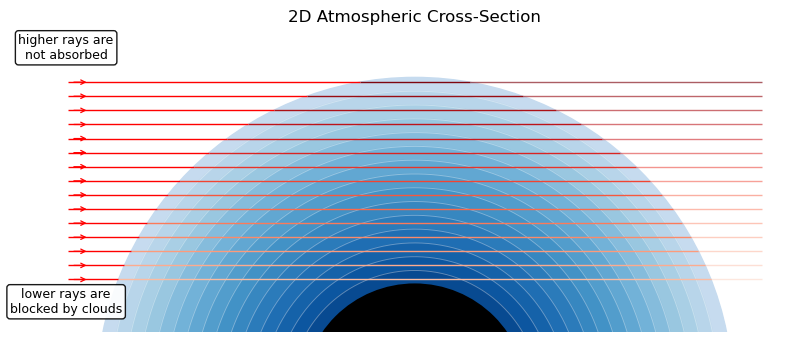
\includegraphics[width=\textwidth]{atmospheric_cross_section.png}
	\caption{Diagram illustrating the radiative transfer process in an exoplanet atmosphere.}
	\label{Fig:RadiativeTransferDiagram}
\end{figure}
We calculate attenuation of the incoming ray, which is written in equation \ref{Eq:RadiativeTransfer} \cite{Bouguer1729} as a function of the optical depth $\tau_\lambda$ along the ray, where $I_{\lambda,0}$ is the incoming specific intensity from the star, $s$ is the distance along the ray, and $\tau_\lambda$ is the optical depth.
\begin{equation}
	I_\lambda(s) = I_{\lambda,0} e^{-\tau_\lambda(s)}
	\label{Eq:RadiativeTransfer}
\end{equation}
If $\tau_\lambda \ll 1$ the atmosphere is mostly transparent at that wavelength; if $\tau_\lambda \gg 1$ the ray is mostly blocked.

The script then builds the wavelength-dependent optical depth from small path elements using the relation in equation \ref{Eq:WavelenghtDependantOpticalDepth} \cite{Brown2001} where $\kappa_\lambda$ is the mass absorption coefficient, $\rho$ is the density, $n_i$ is the number density of species $i$, and $\sigma_{\lambda, i}$ is its absorption cross section.
\begin{equation}
	d \tau_\lambda = \kappa_\lambda\,\rho\, ds = \sum_i n_i\,\sigma_{\lambda, i}\, ds
	\label{Eq:WavelenghtDependantOpticalDepth}
\end{equation}
Each pressure layer contributes an amount of absorption set by how many particles are present and how strongly they absorb at that wavelength. 
Summing these contributions along the full ray of light, which is done at the end of the pre-processing phase, gives $\tau_\lambda$ for that impact parameter.
The code snippet in Figure \ref{Fig:TransitDepthCode} shows how the script integrates the contributions from each layer to calculate the transit depth at each wavelength, which is the final output of this part of the code.
\begin{figure}[htb!]
\centering
\begin{lstlisting}[language=Python]
for i in range(len(r)-1):
	if (r[i] >= Rp):
		integral_gt_Rp[:] += 0.5*((r[i]*(1.0 - exptau[i, :]) + (r[i+1]*(1.0 - exptau[i+1, :])))*(r[i+1] - r[i]))
	if (r[i] < Rp):
		integral_lt_Rp[:] += 0.5*((r[i]*(exptau[i, :]) + (r[i+1]*(exptau[i+1, :])))*(r[i+1] - r[i]))
transit_depth[:] = (Rp*Rp + 2.0*integral_gt_Rp[:] - 2.0*integral_lt_Rp[:])/(Rs*Rs)
\end{lstlisting}
\caption{Transit Depth Calculation Code}
\label{Fig:TransitDepthCode}
\end{figure} 
\subsection{Pressure Grid and Hydrostatic Equilibrium}
\label{Section:Hydrostatic}
The code represents the exoplanet atmosphere as a 1D logarithmic pressure grid from P = $10^{-4}$Pa to $10^{7}$Pa.
This range covers the pressures probed probed in transmission spectroscopy, from the thin upper atmosphere to the deeper layers where clouds or surfaces may exist \cite{Madhusudhan2009-ir}.
While it could be argued that the limit for high pressure is too great, as it is unrealistic that we would be able to probe such depths, we believe it is necessary to ensure that the cloud deck is included in the grid for cases where $P_\mathrm{cloud}$ is high.
For these cases however, the large amount
For each pressure level $P_j$ it assigns a temperature ($T_j$) using equation \ref{Eq:T_j=T_pP_j}, where $T_p$ is a reference temperature and $P_j$ is the pressure at that level, and number density using the ideal gas law equation \ref{Eq:IdealGas}.
\begin{equation}
	T_j = T_p P_j
	\label{Eq:T_j=T_pP_j}
\end{equation}
To know how far rays travel through each layer, we need to find the radius $r$ at each pressure level.
This is obtained by integrating the equation of hydrostatic equilibrium, $ \frac{\mathrm{d}P}{\mathrm{d}r}$, which leads to the expression in equation \ref{Eq: dr = dlnP}.
\begin{equation} 
	dr = - \frac{k_BT}{\mu g}dlnP
	\label{Eq: dr = dlnP}
\end{equation}
The calculation of gravity relative to radius, where $g_\mathrm{ref}$ is the surface gravity at a reference pressure $P_\mathrm{ref}$ and $r_\mathrm{ref}=R_\mathrm{p}$ is the corresponding radius, is stated in equation \ref{Eq:Gravity},
\begin{equation}
	g(r) = g_\mathrm{ref} \left(\frac{r_\mathrm{ref}}{r}\right)^2
	\label{Eq:Gravity}
\end{equation}
From this reference point, the script steps outwards and inwards in even steps of $\log P$ to build the arrays $r(P_j)$ and $g(P_j)$. 
This converts the original pressure grid into a grid of atmospheric shells.

We then set the composition of the atmosphere in terms of logarithmic mixing ratios $(\log_{10} X_i)$ for each molecule. 
This was calculated as a typical sub-neptune's composition [INSERT REFERENCE TO HARRIETS SECTION ON SUB NEPTUNE COMPOSITION CALCULATION]. 
From these mixing ratios, the mean molecular weight is calculated as $\mu = \sum_i X_i\,m_i$.

The absorption cross sections $(\sigma_{\lambda,i}(P,T))$ are loaded as arrays and we use RegularGridInterpolator \cite{Scipy2020} to evaluate the cross sections at the pressures and temperatures of the model atmosphere and at the wavelengths of interest. 
For each wavelength $\lambda_k$ and layer $j$, the total absorption per unit path length is then calulated in equation \ref{Eq:TotAbsoptionPerUnitLength}.

\begin{equation}
	\sum_i n_{i,j} \, \sigma_{\lambda_k,i}(P_j,T_j) = n_j \sum_i X_i\,\sigma_{\lambda_k,i}(P_j,T_j)
	\label{Eq:TotAbsoptionPerUnitLength}
\end{equation}

\subsection{Collision-Induced Absorption}
\label{Section:CIA}
The script also accounts for collision-induced absorption (CIA) from H$_2$--H$_2$ and He--H$_2$ pairs.
H$_2$ has no permanent dipole moment, However, during a collision between molecules the electron clouds of the pair are briefly distorted, creating an induced dipole that can form a momentary bond between the molecules \cite{Richard2012}.
This is known as london dispersion forces and is a key mechanism for absorption in H$_2$-rich atmospheres.
This short-lived collision pair can absorb radiation in the wavelength we are observing.

This phenomenon is important in H$_2$-rich atmospheres, where the absorption line from H$_2$ alone is weak but the CIA contribution can become significant as it scales with the square of the number density.
Unlike molecular absorption lines, which are narrow and defined, collision-induced absorption produces a broad and smooth absorption band as collisions have a range of random separations and interaction geometries rather than a single bound-state transition like a typical molecular line.
As a result, collision-induced absorption often fills in spectral windows between strong molecular bands which makes detecting these molecules more difficult. This is important for our project as we are looking for ideal sub-neptune tagets to study the atmospheres of.

Because CIA requires two molecules to interact, its contribution to $\tau_\lambda$ is proportional to the collision rate of the molecules and therefore scales with the square of the number density for H$_2$--H$_2$ and the product of the number densities for He--H$_2$ \cite{Freedman2008}.
For a background gas with total number density $n_j$ and mixing ratios $X_i$, this gives a quadratic relationship ($\propto n_j^2$) as seen in equation \ref{Eq:CIA} where $\sigma_{\lambda}^{\mathrm{H_2-H_2}}$ and $\sigma_{\lambda}^{\mathrm{He-H_2}}$ are the CIA cross sections for H$_2$--H$_2$ and He--H$_2$ pairs respectively.
\begin{equation} 
	\tau_{\lambda}^{\mathrm{CIA}} \propto n_j^2\,X_{\mathrm{H_2}}^2\,\sigma_{\lambda}^{\mathrm{H_2-H_2}} + n_j^2\,X_{\mathrm{H_2}}X_{\mathrm{He}}\,\sigma_{\lambda}^{\mathrm{He-H_2}}
	\label{Eq:CIA}
\end{equation}
While initially looking intimidating, the CIA absorption is actually simple to calculate. 
The two halves of equation \ref{Eq:CIA} are the contributions from the two types of collisions. Each half is reminiscent of equation \ref{Eq:WavelenghtDependantOpticalDepth} where we find the contribution is proportional to the cross section.
Since $n_j = \frac{P_j}{k_B T_j}$ (equation \ref{Eq:IdealGas}), CIA generally becomes more important at higher pressure, where collisions are more frequent \cite{Richard2012}.

Due to CIA having a low probability of absorption per collision, it is often negligible in low abundance gases, which is why we only include it for H$_2$--H$_2$ and He--H$_2$ pairs in our model, as these are the dominant molecules in a sub-neptune atmosphere and therefore have the highest collision rates.

After these CIA terms are added to the wavelength-dependent molecular opacity, the code holds a 2D array opacity[k,j] representing $\sum_i n_{i,j}\sigma_{\lambda_k,i}$ for each wavelength and pressure level.

\subsection{Slant Optical Depth and Transit Integration}
\label{Section:SlantAndTransit}
Given the radial grid $r_j$ and the opacity at each layer, the next part of our script finds the optical depth $\tau_\lambda(r)$ along rays that pass through the planet at different layers $r$. 
For a ray with minimum radius $r_i$, the path length through layers at larger radii is set by equation \ref{Eq:PathLength} so that the path length across a shell between $r_j$ and $r_{j+1}$ is $\Delta s_j = s(r_{j+1}) - s(r_j)$.
\begin{equation}
s(r) = \sqrt{r^2 - r_i^2}
\label{Eq:PathLength}
\end{equation}
The code loops over the layers above each impact parameter and approximates the slant optical depth by the sum \ref{Eq:SlantOpticalDepth} where the opacity is averaged between adjacent layers to obtain an estimate \cite{Brown2001}.
\begin{equation}
	\tau_\lambda(r_i) \approx \sum_j \left[\frac{\mathrm{opacity}_{k,j} + \mathrm{opacity}_{k,j+1}}{2}\right] \Delta s_j
	\label{Eq:SlantOpticalDepth}
\end{equation}

If the pressure at a given radius exceeds the prescribed cloud-top pressure $P_\mathrm{cloud}$, a very large additional optical depth (e.g. $\tau\sim 10^3$) is added to mimic an effectively opaque cloud deck.

The fraction of light transmitted along that ray is $e^{-\tau_\lambda(r_i)}$.  The script converts this to an effective transit radius with the formula for transmission spectroscopy in equation \ref{Eq:TransitDepth} \cite{Seager2000,Brown2001}.

\begin{equation}
	\Delta_\lambda = \frac{\pi R_\mathrm{p}^2 + 2\int_{r>R_\mathrm{p}}  r \bigl[1 - e^{-\tau_\lambda(r)}\bigr]\,\mathrm{d}r 
	- 2\int_{r<R_\mathrm{p}} r\,e^{-\tau_\lambda(r)}\,\mathrm{d}r}{\pi R_\mathrm{s}^2}.
	\label{Eq:TransitDepth}
\end{equation}

The first term is the area the opaque disk of radius $ R_\mathrm{p} $. 
The second term adds the atmosphere above this.
The third term subtracts light that is able to pass through layers that are inside $ R_\mathrm{p} $ but not completely opaque.
These integrals are then evaluated using the $ r_i $ grid and the precomputed values of $ e^{-\tau_\lambda(r_i)} $.

The code for this final section of the pre-processing phase is seen in figure \ref{Fig:TransitDepthCode}.

\bibliographystyle{unsrtnat}
\bibliography{references}

\end{document}